
This section follows the ideas presented in~\cite{Kornysheva2014}. 
Generally, we are to determine how different the reaction of voxels to different combinations of conditions. 
Machine learning studies different algorithms that are able to find regularities within object's features in order to extract some information about the object. In particular, classification problem is to train a classifier, a function that maps features of the object to the class that this object belongs to. 

\subsection{K-Nearest-Neighbors (KNN) classifier}

\begin{figure}[ht]
\centering
\begin{minipage}[c]{0.3\textwidth}
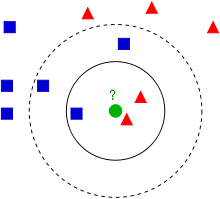
\includegraphics[width=0.9\textwidth]{220px-KnnClassification.png}
\end{minipage}
\begin{minipage}[c]{0.6\textwidth}
\caption{Example of KNN classification. The test sample (green circle) should be classified either to the first class of blue squares or to the second class of red triangles. If K = 3 (solid line circle) it is assigned to the second class because there are 2 triangles and only 1 square inside the inner circle. If K = 5 (dashed line circle) it is assigned to the first class (3 squares vs. 2 triangles inside the outer circle). Credit to https://en.wikipedia.org/wiki/K-nearest\_neighbors\_algorithm\#/media/File:KnnClassification.svg}
\label{fig:knn_example}
\end{minipage}
\end{figure}

One of the simple classifiers is \emph{ K-Nearest-Neighbors} (KNN) classifier, see \autoref{fig:knn_example}.
Given feature vector $x$ and training set $Tr=(\{x_i\},\{c_i\})$ a classical KNN classifier predicts classification label $c$ such that 
$$c^*(x)\;\; := \;\; \arg\max_y \#\{i : x_i \in knn(Tt,x) \;\&\; c_i=y \}$$ where $knn(Tr,x)$ is the set of $K$ nearest neighbors of vector $x$ from the set $\{x_i\}$. The classifier can be used to produce a confidence measure $conf(x,c,Tr)$ that shows the likelihood of test vector $x$ belonging to class $c$:
 $$ conf(x,c,Tr) \;\; := \;\; \frac{\#\{i : x_i \in knn(T,x) \;\&\; c_i=y \}}{K}. $$ The value of $conf(x,c,Tr)$ reaches its maximum value of $1$ if all K nearest neighbors are from class $c$. %$conf(x,c)$ generates a soft score of class $c$ given feature vector $x$.

Given test dataset $R=(\{x'_i\},\{c'_i\})$ where $x'_i$ are feature vectors and $y'_i$ are true class labels, we define the average accuracy (AC) of classification as 
\begin{equation}
AC(R,Tr) \;\; := \;\; \frac1{|R|}\sum_i conf(x'_i, c'_i,R).
\label{eq:ac}
\end{equation}
Note that $AC(Tr)$ is en estimator of probability of correct classification. If accuracy is close to 1 the classifier is able to distinguish feature vectors coming from different classes. That means that features~$x_i$ contain a lot of information about classes $c_i$ they originate from. On the other hand, if features~$x_i$ do not contain relevant information about class $c_i$ the classifier will not be able to predict correct class better than random guessing\footnote{It is in case of balanced data, i.e. the number of representatives of different classes is the same in the training set.}. In this case the accuracy will be $\frac1{|C|}$ where $|C|$ is the number of different classes. 

\subsection{Cross-validation}

\newcommand{\CVAC}{CV\!\!AC}

Cross-validation is a powerful technique that allows to estimate unbiased statistics, e.g. the average accuracy, in situations where the test data is not provided. Suppose that given training set $Tr$ is partitioned into $n$ folds $Tr=\cup_{i=1}^n T_i,$ then \emph{cross-validated average accuracy} is $$\CVAC(Tr) \;\; := \;\; \frac1n\sum_{i=1}^n AC(T_i,Tr \setminus T_i).$$ If the training set is partitioned in a way that folds are independent on each other $\CVAC(Tr)$ is an unbiased estimator of the probability of correct classification.

\begin{figure}[t]\centering
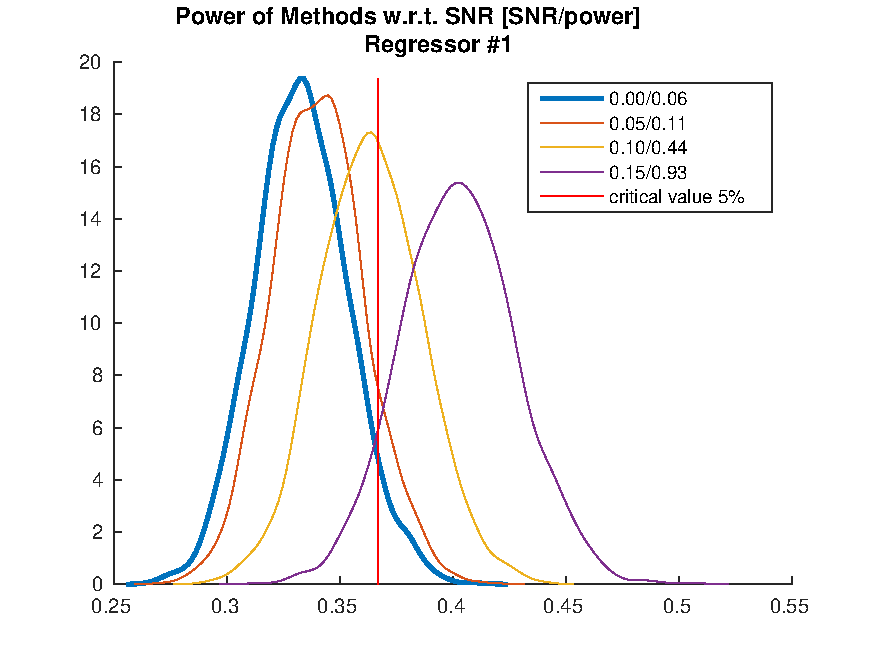
\includegraphics{sample_knn_conv_1}  
\caption{KNN: Estimated distribution (probability densities) of the average accuracy of KNN classifier w.r.t different levels of signal noise ratio (SNR). We test the presence of the main effect against pure noise (bold blue curve). The critical value (red vertical bar) is chosen as $95$ percentile of H0 distribution (bold blue curve). The power is the rate of rejection of H0 in the presence of the main effect. The legend on the plot shows the SNR and power of the statistic test. The power reaches level of $93\%$ at SNR=$0.15$.}\label{fig:knn convergence}
\end{figure}

\subsection{Factorial pattern analysis of fMRI data}

In factorial pattern analysis of fMRI data we are interested in the following question. Does a given region of the brain (represented as activation pattern of voxels) encode information about different conditions and their interaction? One way to answer this question is to train a classifier that predicts the condition that resulted in the observed activation pattern. If the classifier predicts the correct condition significantly better than random guessing then the answer to the question is positive.

In our experimental setting there are 2 factors (T and S), each of them has 3 levels. Each test run measures 9 (one for each combination of factors) activation pattern in 160 voxels. The total number of runs is 6. This yields 54 feature vectors of dimensionality 160. Each run naturally forms an independent fold for cross-validation.

\subsection{Main effect detection}

In this subsection we are interested in detecting the presence of the main effect of a factor. Activation patterns measured under different levels of the factor are significantly different from each other, if the main effect is present. This, in principle, allows a classifier to distinguish the patterns. So, to detect the main effect we train our KNN classifier to predict 3 levels of the factor based on activation patterns. We choose $K=10$ as the one that gives the best performance. \autoref{fig:knn convergence} shows the result of the experiment.

\begin{figure}[t]
\begin{tabular}{cc}
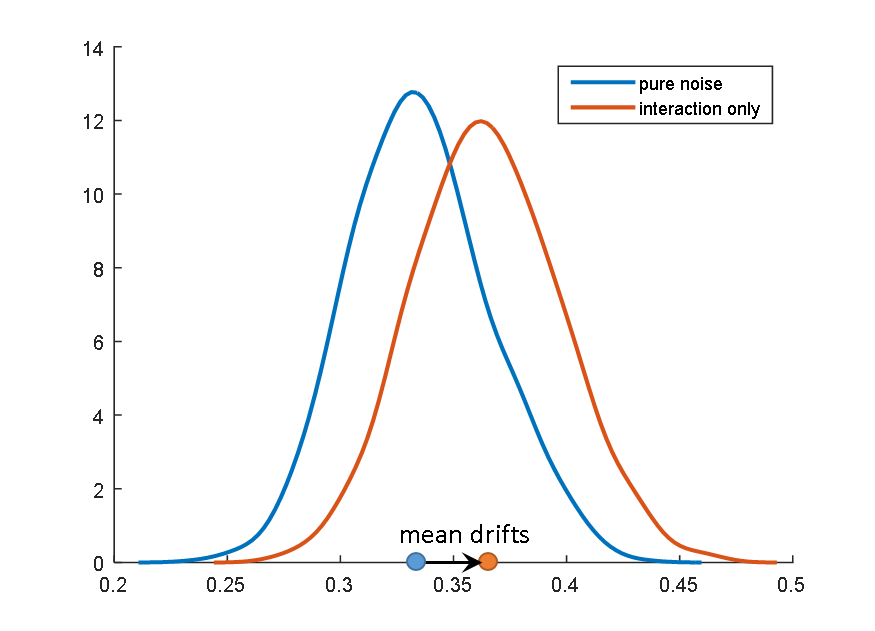
\includegraphics[width=0.5\textwidth]{drift} &
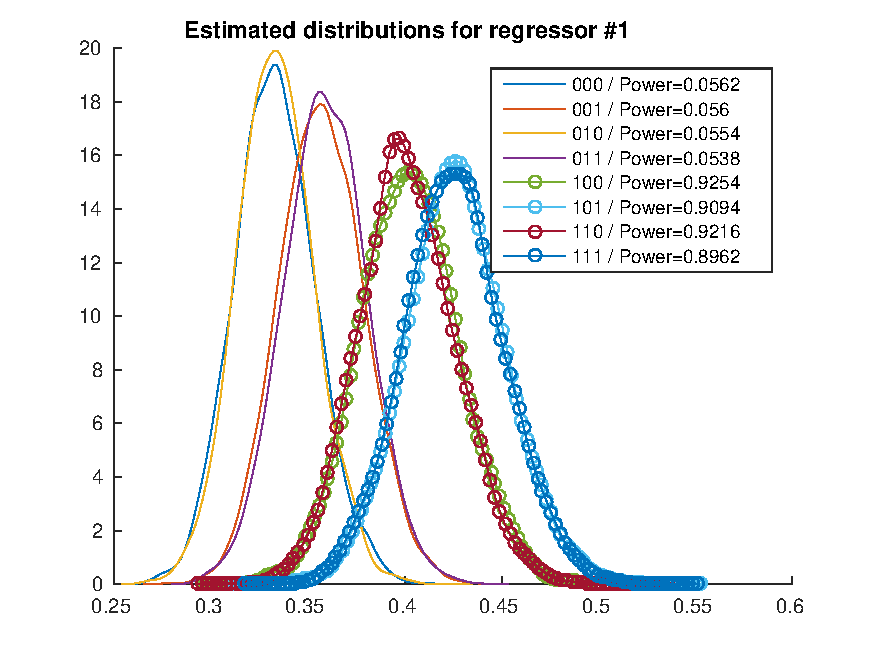
\includegraphics[width=0.5\textwidth]{sample_knn_distributions_1}  \\
(a) & (b) 
\end{tabular}
%\vspace{-6mm}
\caption{KNN: Testing main effect (circle markers) against all possible combinations of other effects (without markers). \newline
{\bf (a)} Note that as soon as some interaction is introduced the expected value of the classification accuracy increases. This is because interaction allows to discriminate different conditions even if no main effect present.\newline
 {\bf (b)} The distribution of the statistic is not invariant to presence of other effects. 0/1 in the legend codes absence/presence of two main effects and interaction between them. Critical value is given by 95\% percentile of H0 distribution. The power is computed as portion of points generated from H1 distribution that are above the critical value.  For example, ``101 / Power = 0.852'' corresponds to H1 s.t. there is no main effect S but there are main effect T and interaction between S and T. H0 in this case is ``001'', i.e. only interaction is present.}\label{fig:knn drift}
\end{figure}

We observe that as we increase the level of interaction the expected cross-validated average accuracy also increases, see \autoref{fig:knn drift}a. The presence of interaction between factors T and S means that there is a unique structure of activation patters that allows distinguishing all 9 possible combinations of the factors significantly better than random guessing. But the ability to decode 9 combinations implies the ability to decode each of the factors. This results in the drift in the average accuracy.

\begin{figure}[t]
\centering
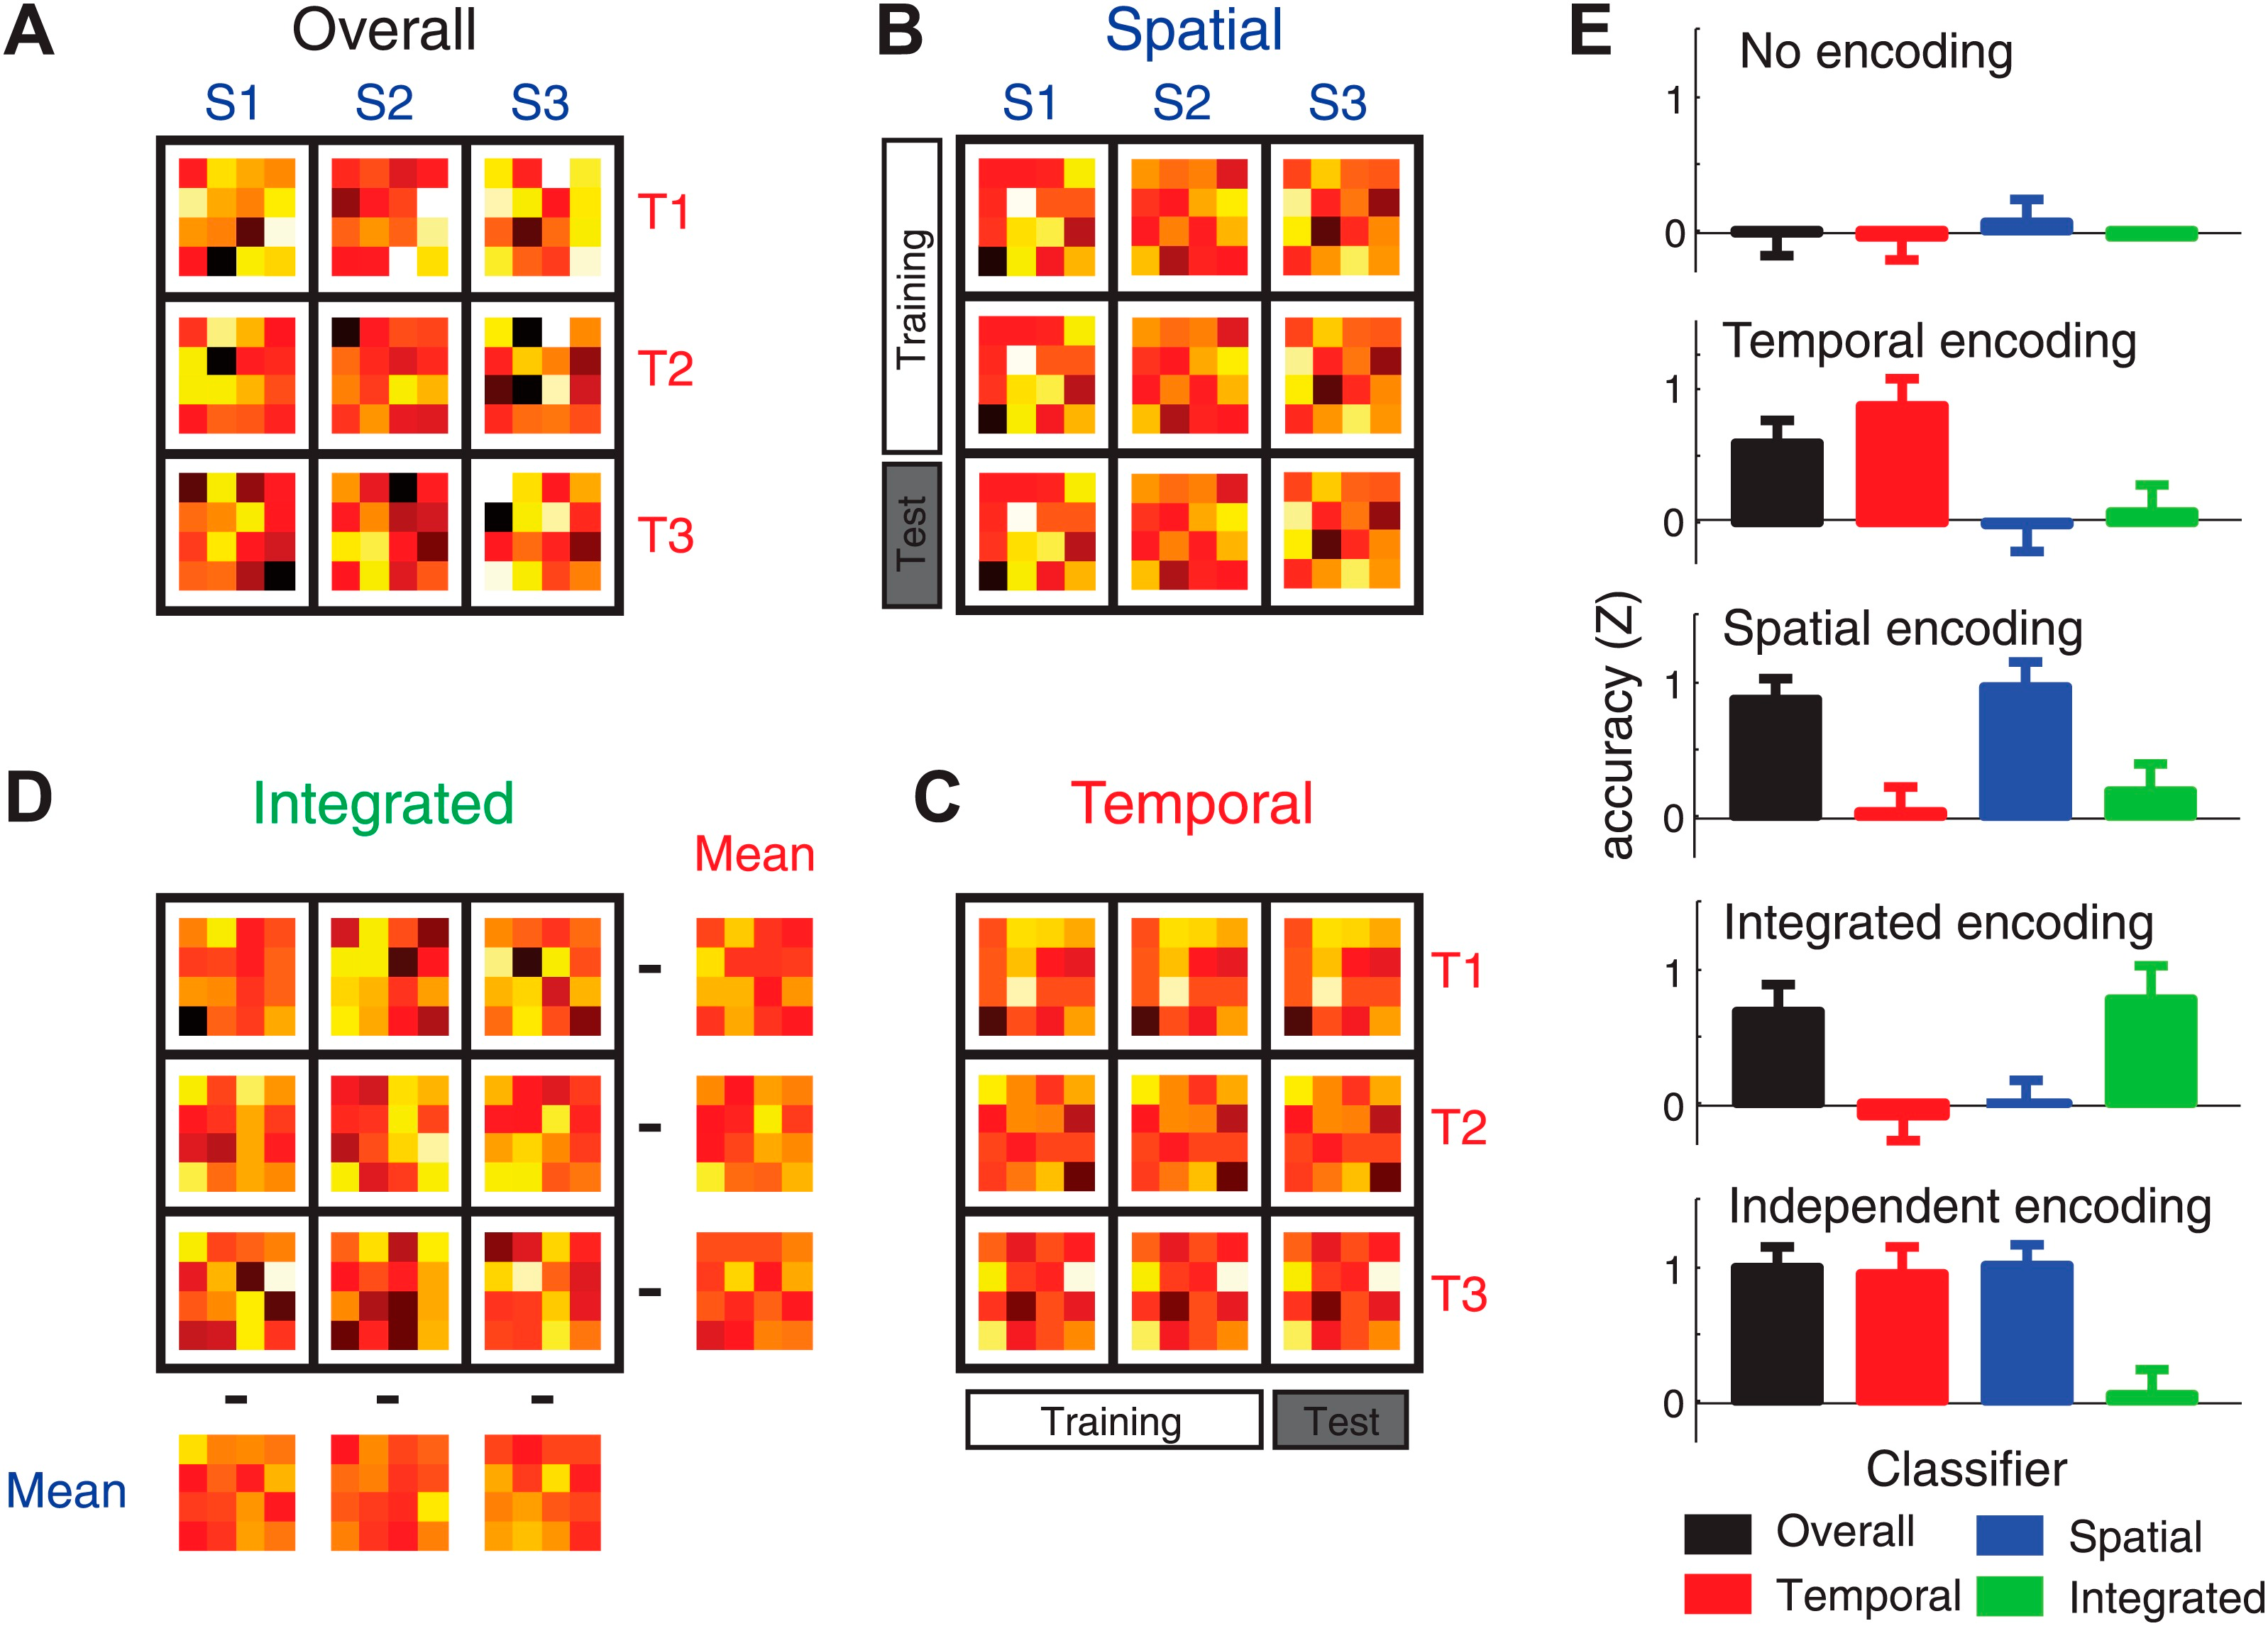
\includegraphics[width=0.60\textwidth,clip=true,trim=0 0 28cm 0]{elife-03043-fig3-v1}
\caption{Two factors have 3 levels: S1,S2,S3 and T1,T2,T3. All possible combination of levels result in 9 measured activation patterns ({\bf A}). Double cross-validation allows to decode the main effects ({\bf B} and {\bf C}) independently from interaction. Mean subtraction for both factors allows to destroy their main effects and detect only interaction ({\bf D}). The plot is by~\cite{Kornysheva2014}}\label{fig:patterns}
\end{figure}

\begin{figure}[ht]
\centering
\begin{minipage}[c]{0.6\textwidth}
\centering
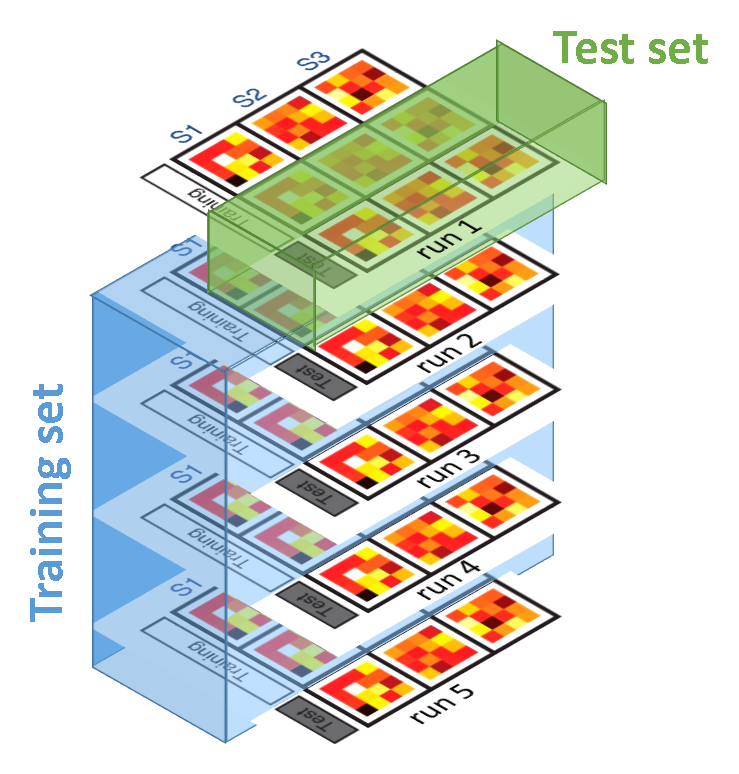
\includegraphics[width=.6\textwidth]{2xval.png}
\end{minipage}\hfill
\begin{minipage}[c]{0.4\textwidth}
\caption{Double cross validation for detecting the main effect of the spatial factor. Suppose one tests a classifier on  patterns that have the temporal factor level of Tn (marked by word test on the plot) and originate from run $i$ (green box on the plot). Then the classifier should be trained on the rest of the patterns except the patterns with the same temporal level Tn or from run $i$ (blue box on the plot).}\label{fig:2xval}
\end{minipage}
\end{figure}

To overcome this issue \cite{Kornysheva2014} propose to use \emph{double cross validation}. See \autoref{fig:patterns}B. Suppose the patterns only contain interaction and there is no main effects. Let's consider the patterns where factor T has the level of Tn. There are three patterns, see lower row in  \autoref{fig:patterns}B. There is a unique structure within this patterns that allows distinguishing between them. How ever the classifier will be able to recognize this structure only if training set contains such combinations of the factors. So, when we test the patterns from factor Tn  we should exclude from the training set the patterns coming from Tn as well, see \autoref{fig:2xval}. This prevents classifier from learning interaction structure while preserves the main effect information, see \autoref{fig:2xval for main effect}.

\begin{figure}[t]
%\begin{subfigure}[t]{0.49\textwidth}
\subfloat[][Testing the main effect for the first factor (circle markers) against all possible combinations (without markers) with double cross-validation. The distributions only depend on the presence of the main effect. Note, there is no drift as in \autoref{fig:knn drift}.]{
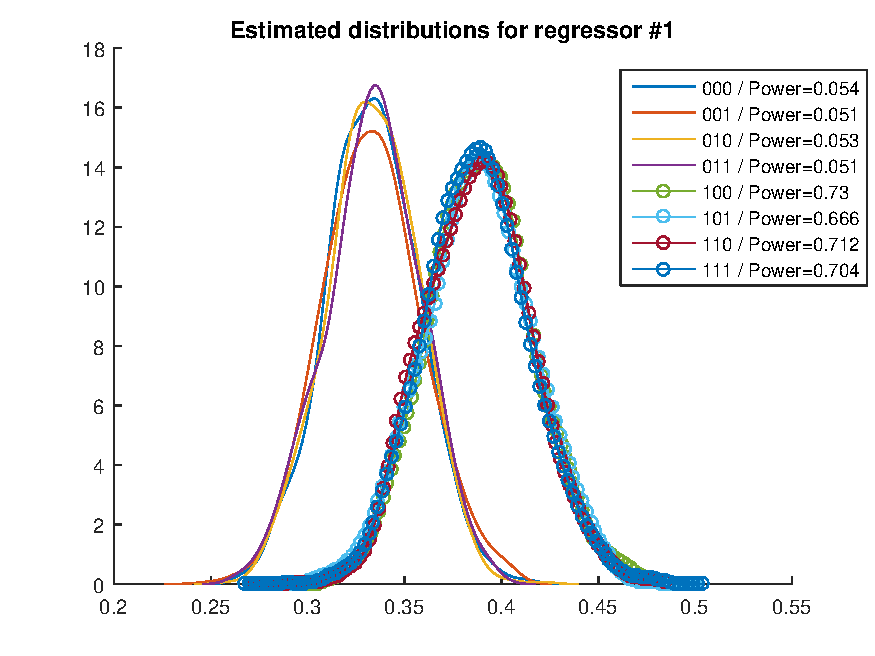
\includegraphics[width=.48\textwidth,clip=true,trim=0 0 0 7.5mm]{sample_knn2_distributions_1}
%\caption{Testing the main effect for the first factor (circle markers) against all possible combinations (without markers) with double cross-validation. The distributions only depend on the presence of the main effect. Note that there is no drift as in \autoref{fig:knn drift}.} 
\label{fig:2xval for main effect}
%\end{subfigure}
}
\hfill
%\begin{subfigure}[t]{0.49\textwidth}
\subfloat[][Testing interaction (circle markers) against all possible combinations (without markers). The distributions only depend on the presence of the interaction.]{
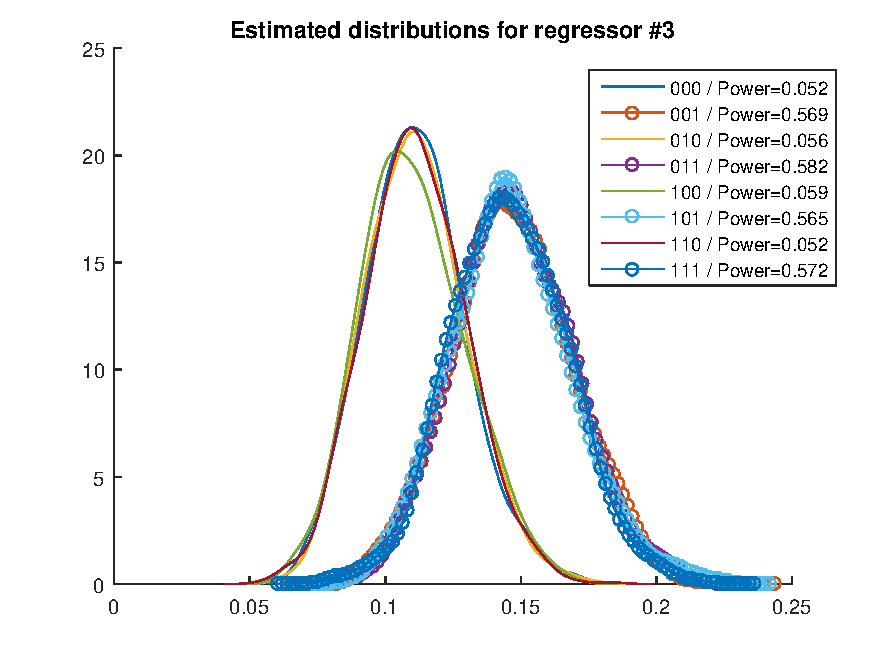
\includegraphics[width=.48\textwidth,clip=true,trim=0 0 0 7.5mm]{sample_knn2_distributions_3}
%\caption{Testing interaction (circle markers) against all possible combinations (without markers). The distributions only depend on the presence of the interaction.} 
\label{fig:test interaction}
}
%\end{subfigure}
\caption{Detection of main effects (a) and interaction (b). Estimated distributions of average accuracy \eqref{eq:ac} are shown. For the legend description see \autoref{fig:knn drift}. The power is worse than in \autoref{fig:knn convergence} due to smaller training set.}
\end{figure}


\subsection{Interaction detection}

To detect interaction  we train a classifier to decode all 9 possible combinations of factor levels. However, if there is no interaction but only main effects the classifier will be able to recognize 9 classes with chances significantly higher than random guessing. \cite{Kornysheva2014} propose to subtract the mean pattern computed withing each factor level, see \autoref{fig:patterns}D. Indeed, the main effect of a fixed factor level is constant and remains the same in the mean pattern. If we subtract the mean pattern we remove main effect from the patterns, see \autoref{fig:test interaction}.

\subsection{Results and conclusions}

\begin{figure}[t]
\subfloat[][Main effect detection with double cross-validation. The power converges to 1 as SNR increases.]{
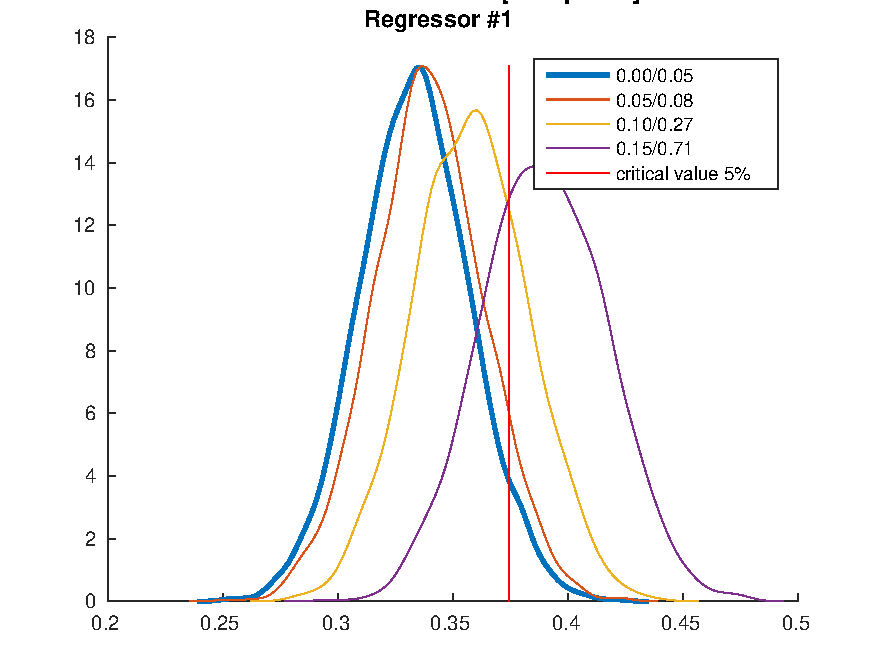
\includegraphics[width=.48\textwidth,clip=true,trim=0 0 0 8mm]{sample_knn2_conv_1}
\label{fig:knn2 convergence:main}
}
\hfill
\subfloat[][Interaction detection with mean subtraction.]{
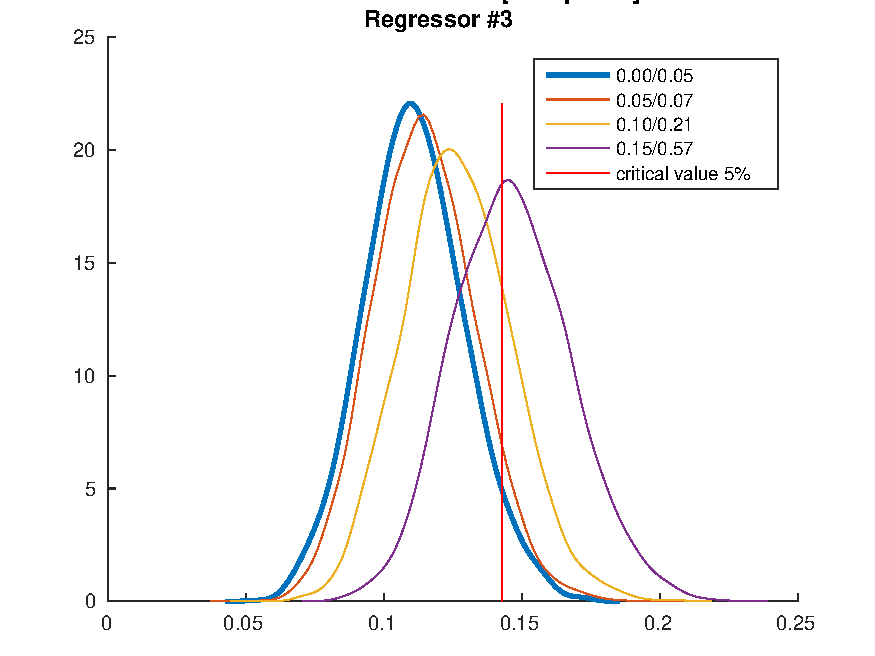
\includegraphics[width=.48\textwidth,clip=true,trim=0 0 0 8mm]{sample_knn2_conv_3}
\label{fig:knn2 convergence:int}
}
\caption{Main effect and interaction detection. Estimated distributions of average accuracy \eqref{eq:ac} are shown. The power rapidly increases as Signal-to-Noise-Ratio (SNR) increases.}
\label{fig:knn2 convergence}
\end{figure}

The classification approach is very powerful technique for decoding the activation patterns. It relies on a very popular and established field of machine learning that allows removing the limitations on the number of voxels and assumption of normality of the data. Our experiments show that the approach allows reliable detection of the main effects and interaction. With SNR level of 0.15 the power of the proposed statistical test (base on average accuracy) reaches the level of $\sim71\%$ for main effect detection (\autoref{fig:knn2 convergence:main}) and $\sim57\%$ for interaction (\autoref{fig:knn2 convergence:int}). We also show that as SNR increases the power of our statistical test reaches 1 very quickly (\autoref{fig:knn convergence}).\autoref{fig:2xval for main effect}  \autoref{fig:test interaction}
